\chapter{\label{ch:2-neutrinophysics}Neutrino Physics} 

%%%%%%%%%%%%%%%%%%%%%%%%%%%%%%%%%%%%%%%%%%%%%%%%%%%%%%%%%%%%%%%%%%%%%%%%%%%%%%%%
% From my COS report

% This chapter will cover details of relevant neutrino physics for the thesis 
% project. The theoretical aspects of neutrino physics will be reviewed 
% including the theory of neutrino oscillations in the PMNS framework. 
% Neutrino production will also be discussed including details of neutrino 
% production in supernovae and the role neutrinos can have in understanding 
% the mechanics of a supernova burst
 
% The work for this section is ongoing as it is associated with the analysis 
% work in the other sections, it is expected to be completed by the end of 
% December 2019.
%%%%%%%%%%%%%%%%%%%%%%%%%%%%%%%%%%%%%%%%%%%%%%%%%%%%%%%%%%%%%%%%%%%%%%%%%%%%%%%%

% TODO TODO TODO TODO TODO TODO TODO TODO TODO TODO TODO TODO TODO
% Decide on historical vs theoretical overview or both
% TODO TODO TODO TODO TODO TODO TODO TODO TODO TODO TODO TODO TODO

% \minitoc

Despite being one of the most abundant particle in the universe, neutrinos are 
some of the most elusive; due to the fact that neutrinos can only interact via
the weak interaction. The history of neutrino physics is therefore strongly
connected to the discovery and study of weak interactions. Measurements by
Chadwick in 1914 showed that the energy spectrum of electrons released in
\(\beta\)--decays was continuous, this is in contrast to discrete spectra
observed in \(\alpha\) and \(\gamma\) decays, and seemingly violates
conservation of energy under the assumption of a two--body final state which was
expected at the time. In order to solve this problem, Pauli postulated that the 
continuous energy spectrum could be explained if the energy released in a 
\(\beta\)--decay could be shared with an additional neutral weakly interacting 
fermion which Pauli named the neutron. Fermi later renamed Pauli's fermion to 
the neutrino, after Chadwick discovered the neutron in 1932. Despite claims that 
neutrinos might never be detected, neutrinos have now been discovered and they 
have been found to have a number of interesting properties which were not 
anticipated when neutrinos were first postulated. This chapter will detail 
some of the history and theory of neutrino's and their interactions.

In this chapter, Section \ref{nu_hist} will give a brief historical overview of 
neutrino physics, Section \ref{nu_osc} will introduce neutrino oscillations
and the theory used to describe them, while Section \ref{nu_prod} will discuss
neutrino interactions in matter as well as neutrino production. Finally Section
\ref{nu_sn} will discuss the production of neutrinos in supernovae, as well as
the role they could play in understanding supernovae.

\section{A Brief History of Neutrino Physics} \label{nu_hist}

The first attempt to incorporate the neutrino into a theoretical model came in
1934 when Fermi presented his theory of \(\beta\)--decay, in this theory the 
neutrino takes part in a four--point interaction with the other components of 
the \(\beta\)--decay interaction \cite{Fermi1934}. The incredible success of this 
theory in explaining the observed properties of \(\beta\)--decays provided 
strong evidence for the neutrinos existence, however, in 1934 after using 
Fermi's theory to predict the strength of neutrino interactions, H. Bethe and 
R. Peierls found that the interactions were so weak that they might never be 
observed, a prediction that held true for over 20 years \cite{Bethe1934}.

The first breakthrough in experimental neutrino physics would come in 1956. F.
Reines and C. Cowan were attempting to measure positrons produced in inverse 
\(\beta\)--decay interactions,
\begin{equation}
	\bar{\nu_e} + p \rightarrow n + e^+.
\end{equation}
A detector containing 1400 litres of liquid scintillator was used to measure the 
large flux of electron anti--neutrinos in the vicinity of the Savannah River 
nuclear reactor. They observed a large increase in the rate of positron events 
when the reactor was on when compared to when the reactor was switched off, the 
first experimental evidence for the existence of neutrinos \cite{Reines1953}. 

The discovery of the electron neutrino opened the door to answer questions of 
neutrino flavour. As neutrinos are produced alongside a charged lepton it is 
natural to compare the properties of neutrinos with their partners in the weak
interaction. At the time of the discovery of the neutrino there were two known
charged leptons, the electron and the muon, and so physicists asked whether the
neutrinos produced alongside muons are different from those produced alongside
electrons. In 1962, Lederman et al discovered the muon neutrino at Brookhaven
National Laboratory; by creating a beam of muon associated neutrinos using 
decaying pions, and observing the leptons produced in neutrino interactions 
after all other particles had been absorbed. They found that only muons where 
produced in the resulting neutrino interactions, and therefore the neutrinos 
produced were only ever associated with a muon, which shows that neutrinos are 
produced with a distinct flavour in weak interactions \cite{Danby1962}.

In 1973 the Gargamelle experiment at CERN released results on the measurement of
neutrino interactions \cite{Hasert1973}. They observed a new type of 
interaction, neutral current (NC) interactions: 
\begin{equation}
	\nu_l + N \rightarrow \nu_l + X
\end{equation}
which are characterised by the lack of an observable charged lepton in the final
state. Unlike charged current (CC) interactions, which are mediated by the 
charged W boson, these NC interactions are mediated by the neutral 
\(\mbox{Z}^0\) boson.

With the discovery of the tau--lepton in 1977 it was expected that there should 
be an associated tau neutrino, however, it wouldn't be detected until 2001 by 
the DONUT experiment \cite{Kodama2001}. In the experiment, tau neutrinos where 
produced from the decay of charmed mesons produced in collisions between protons 
and a stationary target. The neutrino interactions where detected in emulsion 
detectors, where the unique geometry of the interaction, in which a short tau 
track is produced at the vertex followed by a long muon track, allowed them to 
be distinguished from other decays.

While additional neutrino species are possible, data from measurements of the Z 
boson line--shape at LEP in 1992 restricts the number of active light neutrino 
species to be three \cite{LEP1992}. An active light neutrino is any neutrino 
with \(m_\nu < \frac{m_Z}{2}\) that can interact with the Z boson, such that the 
decay \(Z \rightarrow \nu \nu \) is possible.

Alongside the discovery of three different types of neutrino, there were
interesting results when observing neutrinos produced in the Sun. The flux of
neutrinos from the Sun at the earth surface had been predicted with Bachall's 
Standard Solar Mode, however, in 1968 when Davis et al measured the flux in the
Homestake experiment they found a deficit with respect to the prediction of the
standard solar model (SSM) \cite{Davis1968, Bahcall1968}, the so called solar neutrino 
problem. In the Homestake experiment electron neutrinos where being measured via 
there inverse beta decay interactions with the chlorine in the target,
\begin{equation}
	v_e + ^{37}\mbox{Cl} \rightarrow ^{37}\mbox{Ar} + e^-.
\end{equation}
The neutrino interaction rate was measured by counting the number of argon 
atoms in the chlorine tank by capturing them on helium gas which was
periodically bubbled through the chamber.

In addition to the solar neutrino problem, a similar deficit was observed in
1988 for muon neutrinos produced during cosmic ray showers in the atmosphere.
The Kamiokande experiment was able to measure both electron and muon neutrino 
interactions via the cerenkov radiation produced by the charged leptons in 
water, their data was consistent with the expected rate of electron neutrinos 
from the atmosphere, however, a deficit of muon neutrinos was observed
\cite{Hirata1988}. 

The next generation of the Kamiokande experiment, Super Kamiokande, aimed to
understand the observed deficit of atmospheric muon neutrinos with a larger 
water cerenkov detector capable of resolving the angular distribution of 
atmospheric neutrino interactions. Super Kamiokande consists of a cylindrical 
vessel containing 50kt of ultra pure water, surrounded by an array of around 13
,000 photomultiplier tubes to detect the cerenkov light. Electron and muon 
neutrinos can be distinguished based on the pattern of cerenkov light that is 
left in the detector; due to their higher mass muons leave clear cerenkov 
rings in the detector while electrons, which can scatter and shower, tend to 
leave diffuse "fuzzy" rings on the wall of the detector. In 1998, Super 
Kamiokande published measurements of the flux of atmospheric muon neutrinos as 
a function of azimuthal angle \cite{Fukuda1998}. Since these neutrinos are created a 
short distance from the earths surface, the incoming angle of the neutrino can 
be used to estimate the distance travelled by the neutrino before arriving at 
the detector; the down--going neutrinos have only travelled a short distance in 
the atmosphere (\(\sim 10\mbox{km}\)), while the up--going neutrinos have 
travelled through the entire earth to reach the detector (\(\sim 13,000\mbox{km
}\)). Figure \ref{fig:sk_flux}, shows the flux of neutrinos measured by Super 
Kamiokande as a function of distance travelled; the muon neutrino flux is 
consistent with the no oscillation prediction at small \(\mbox{L} / \mbox{E}_\
nu\), however, for large \(\mbox{L} / \mbox{E}_\nu\) a clear deficit is 
observed. 

\begin{figure}

	\centering

	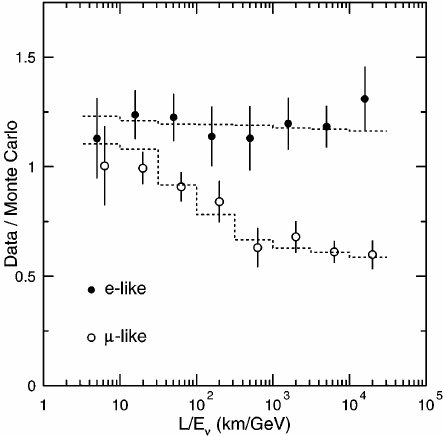
\includegraphics[width=0.7\textwidth]{figures/sk_flux.jpg}

	\caption
	[Ratio of data to Monte Carlo for electron and muon neutrino fluxes 
	measured by the Super Kamiokande experiment as a function of 
	\(\mbox{L} / \mbox{E}_\nu\).]
	{Ratio of data to Monte Carlo for electron and muon neutrino fluxes measured 
	by the Super Kamiokande experiment as a function of 
	\(\mbox{L} / \mbox{E}_\nu\). The Monte Carlo prediction is based on the
	assumption of no oscillations. The muon neutrino flux is consistent with the
	no oscillation prediction at small \(\mbox{L} / \mbox{E}_\nu\), however, for
	large \(\mbox{L} / \mbox{E}_\nu\) a clear deficit is observed. The best fit
	under the assumption of atmospheric (\(\nu_\mu \rightarrow \nu_\tau\))
	oscillations is shown, the best fit parameters are \(\Delta m^2 = 2.2 \times
	10^{-3} \mbox{eV}^2\), and \(sin^22\theta = 1\) \cite{Fukuda1998}.}

	\label{fig:sk_flux}

\end{figure}

While it wouldn't completely solve the solar neutrino problem, the Sudbury
Neutrino Observatory (SNO) was able to provide unique insight into the observed
solar neutrino fluxes in 2002. Unlike other water cerenkov detectors, SNO 
was filled with heavy water, \(\mbox{D}_2\mbox{O}\), instead of its lighter 
isotope. The use of heavy water in the detector gives rise to additional 
neutrino interactions which allowed the SNO experiment to distinguish between 
three different interaction modes: charged current (CC), neutral current (NC), 
and elastic scattering (ES). Each interaction mode is sensitive to different 
parts of the solar neutrino flux, including some sensitivity to the muon 
neutrino and tau neutrino fluxes via the NC and ES interactions. Analysis of the 
data for each of the three unique interaction modes lead to a measurement of 
the flavour composition of the solar neutrino flux at earth, while also 
measuring an overall neutrino flux at earth that is consistent with the SSM.
Figure \ref{fig:sno_flux} shows the composition of the solar neutrino flux as 
measured in the SNO experiment \cite{Ahmad2002}, the flux prediction based on 
the measured rate of NC events is consistent with the predictions of the 
SSM. The composition of solar neutrinos measured in the SNO experiment is not
a result of neutrino oscillations, instead it is the result of matter effects on
the neutrino propagation via the Mikheyev–Smirnov–Wolfenstein (MSW) effect.
However at the time a number of solutions were still possible: MSW conversion,
decoherence, neutrino decay, and others \cite{Smirnov2016}. 

\begin{figure}

	\centering

	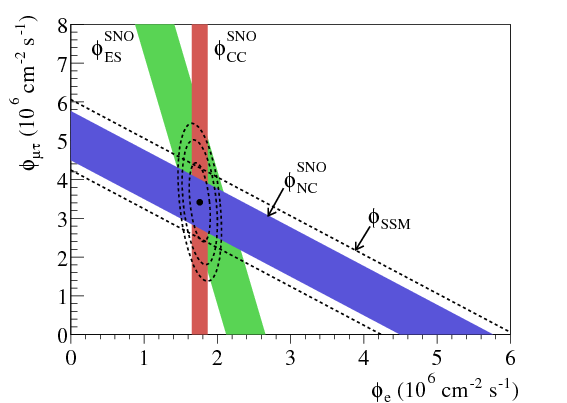
\includegraphics[width=0.8\textwidth]{figures/sno_flux.png}

	\caption
	[Solar neutrino flux composition as measured by the SNO experiment.]
	{Solar neutrino flux composition as measured by the SNO experiment. The
	coloured bands represent the measured flux of charged current (CC),
	neutral current (NC), and elastic scattering (ES) events, including a \(\pm 1
	\sigma\) spread. The central contours represent 68\%, 95\%, and 99\%
	probability contours for the joint \(\phi_e\) and \(\phi_{\mu \tau}\) fit. The
	dashed lines represent the predicted flux of \(^8\mbox{B}\) neutrinos based on 
	the standard solar model \cite{Ahmad2002}. }

	\label{fig:sno_flux}

\end{figure}

In order for neutrino oscillations to be the unique solution to the problem, 
an \(\mbox{L/E}_\nu\) dependence would have to be measured. To make this 
measurement a much shorter neutrino baseline would be needed, along with a 
source of neutrinos with a small energy spread, and a detector with good 
energy resolution. In 2002 the Kamioka Liquid Scintillator Anti--neutrino 
Detector (KamLAND) experiment measured \(\bar{\nu_e}\) oscillations from a 
number of nuclear reactors, which produce neutrinos at the MeV scale \cite{
	Eguchi2003, Araki2005}. Along with an overall deficit of neutrino events, 
they were able to use the high energy resolution of the KamLAND detector to 
measure an \(\mbox{L/E}_\nu\) dependence of the \(\bar{\nu_e}\) survival 
probability.  Figure \ref{fig:kamland_spectrum}, shows the ratio of the 
observed neutrino flux with the no oscillation predicted flux as a function of 
\(\mbox{L/E}_\nu\), a clear dependence can be seen and this data was enough to 
prove that neutrino oscillations were the unique solution to the solar 
neutrino problem.  
\begin{figure}

	\centering

	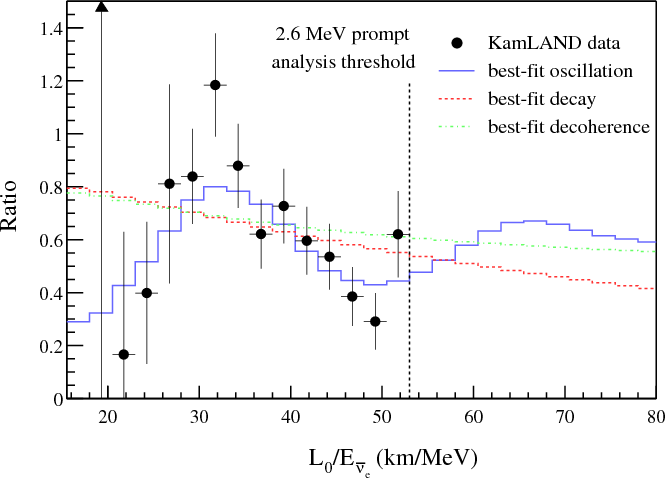
\includegraphics[width=0.8\textwidth]{figures/kamland_spec.png}

	\caption
	[Ratio of observed neutrino flux to the predicted flux in the absence of
	neutrino oscillations in the KamLAND experiment.]
	{Ratio of observed neutrino flux to the predicted flux in the absence of
	neutrino oscillations in the KamLAND experiment as a function of 
	\(\mbox{L/E}_\nu\). The data are fit with three different models: the red 
	dashed line represents the best fit to a neutrino decay model, the green 
	dashed line is for a decoherence model, and the solid blue line represents the 
	best fit of the data to a neutrino oscillation model. The neutrino oscillation
	model, which has a different shape to the other two models, is found to give 
	the best fit to the data \cite{Araki2005}.} 

	\label{fig:kamland_spectrum}

\end{figure}

Based on the results of the above experiments, it was assumed that electron and
muon type neutrinos where oscillating into tau type neutrinos which where then
left undetected. The first evidence of tau neutrino production in oscillations
wouldn't be found until 2010, when the OPERA experiment would measure
a \(\nu_\tau\) candidate in a \(\nu_\mu\) beam. They used similar emulsion 
detectors to those used to discover the \(\nu_\tau\) in DONUT, and a muon
neutrino beam on a 730km baseline from CERN to LNGS. By the end of the 
experiment a total of 10 candidate events have been observed, a total of 6.1 
\(\sigma\) above the background \cite{Agafonova2010, Agafonova2018}.

Since the discovery of neutrino oscillations, many more experiments have made
measurements of neutrino oscillations and placed constraints on the majority of
the parameters of the neutrino oscillation models. Important results of these 
experiments for constraining the parameters of the neutrino oscillation models 
will be highlighted in Section \ref{nu_osc}, along with the theoretical 
overview of neutrino oscillations.

Neutrino oscillations are currently the only measured effect that is not
explained in the SM, and their observation proves that neutrinos are massive.
However, the absolute mass of neutrinos is still unknown because oscillation
experiments are only sensitive to the squared mass differences between the
neutrino mass eigenstates. The question of absolute neutrino mass, is one of a
number of open questions in neutrino physics. The main open questions at the
time of writing are:
\begin{itemize}
	\item What are the absolute masses of the neutrinos?
	\item What is the mass ordering of the neutrino mass eigenstates?
	\item Is there CP violation in the neutrino sector?
	\item Are neutrinos Dirac ($\nu \ne \bar{\nu}$) or Majorana 
		($\nu = \bar{\nu}$) particles?
\end{itemize}

\section{Neutrinos in the Standard Model} \label{nu_sm}

In the standard model neutrinos form part of the left handed fermion doublets
\begin{equation}
	\psi_i = \begin{pmatrix} \nu_i \\ l^-_i \end{pmatrix}
\end{equation}
where they are paired with a charged lepton of the same flavour in charged
CC interactions, and $i$ represents any of the three known generations of 
fermions. Their interactions with other particles in the standard model is
determined by the electroweak (EW) theory, which is derived from the $SU(2)
\times U(1)$ gauge group. The neutrino fields enter into the SM Lagrangian in
the CC and NC interactions:
\begin{align}
	\label{eqn:cc_lag}
	\mathcal{L}^{CC} &= -\frac{g}{2\sqrt{2}}\; j^{CC}_\alpha(x)\; W^\alpha(x)\; +\; h.c. \\
	\mathcal{L}^{NC} &= -\frac{g}{2cos\theta_W}\; j^{NC}_\alpha(x)\; Z^\alpha(x)\; +\; h.c.
\end{align}
Here 
\begin{equation}
	\label{eqn:cc_curr}
	j^{CC}(x) = 2 \sum_{l=e,\mu,\tau} \bar{\nu_l}_{i}(x)\; \gamma_\alpha\; l^i(x)
\end{equation}
is the leptonic charged current and
\begin{equation}
	j^{NC}(x) = \sum_{l=e,\mu,\tau} \bar{\nu_l}_i(x)\; \gamma_\alpha\; \nu_l^i(x)
\end{equation}
is the neutrino neutral current, $W^\alpha(x)$ and $Z^\alpha(x)$ are the vector
boson fields for the $W^\pm$ and $Z^0$ bosons respectively, $g$ is the 
electroweak coupling constant, and $\theta_W$ is the Weinberg angle.

Mass is included in the standard model through the Dirac mass term in the
Lagrangian
\begin{align}
	\mathcal{L}^{D} &= m_D \bar{\psi} \psi \\
	&= m_D \overline{(\psi_L + \psi_R)}(\psi_L + \psi_R) \\ 
	&= m_D(\bar{\psi}_L \psi_R + \bar{\psi}_R \psi_L)
\end{align}
where $L$ and $R$ represent the left and right handed components of the field.
The lack of right handed neutrino states in the standard model therefore means
neutrinos are assumed to be massless in the model. For massive neutrinos to
exists the standard model needs to be modified; right handed neutrino fields
need to be introduced. In addition it is still unknown whether neutrinos are
Dirac or Majorana particles, meaning that additional Majorana mass terms are
possible. A more general neutrino mass term including both Dirac and Majorana
components is 
\begin{equation}
	\mathcal{L}^{D+M} = 
	\begin{pmatrix} \bar{\nu}_L \; \bar{\nu}_R \end{pmatrix} 
	\begin{pmatrix} m_L \; m_D \\ m_D \; m_R \end{pmatrix} 
	\begin{pmatrix} \nu_L \\ \nu_R \end{pmatrix}.
\end{equation}

\section{Neutrino Oscillations} \label{nu_osc}
%%%%%%%%%%%%%%%%%%%%%%%%%%%%%%%%%%%%%%%%%%%%%%%%%%%%%%%%%%%%%%%%%%%%%%%%%%%%%%%%
% TODO
% add in important/latest measurements of osc parameters
%%%%%%%%%%%%%%%%%%%%%%%%%%%%%%%%%%%%%%%%%%%%%%%%%%%%%%%%%%%%%%%%%%%%%%%%%%%%%%%%

Neutrino oscillations are a result of quantum mechanical interference between
different massive neutrino eigenstates. These mass eigenstates are produced and 
measured coherently because the energy and momenta of the neutrino states are
not measured with enough precision to distinguish the mass eigenstate of the
neutrino.

Neutrinos are produced in a state of definite flavour, \(l = e, \mu, \tau\), in 
charged current (CC) and neutral current (NC) weak interactions, 
\begin{equation}
	W^+ \rightarrow l^+ \nu_l, \quad  W^- \rightarrow l^- \nu_l, \quad  Z   \rightarrow \nu_l \bar{\nu_l}.
\end{equation}
The CC processes are mostly used in neutrino oscillation experiments because
they give information about the initial flavour state of the neutrinos. These
processes are governed by the Lagrangian of the CC leptonic interactions, as in
equation \ref{eqn:cc_lag}. The leptonic current \(j^\alpha\) is given in 
\ref{eqn:cc_curr}. The neutrino flavour states, $\nu_l$, can be represented as a 
superposition of massive neutrinos in any case where the energy and momentum 
of the neutrino is not known with enough precision to determine the neutrino 
mass,
\begin{equation}
	\nu_l = \sum_{k} U^*_{lk} \nu_k
\end{equation}
where $\nu_k$ are the neutrino mass eigenstates, and U is a unitary mixing
matrix.

\section{Neutrino Interactions} \label{nu_prod}

\section{Supernova Neutrinos} \label{nu_sn}
